\chapter{Modelo matemático}
\cleanchapterquote{In mathematics, you don’t understand things. You just get used to them.}{John von Neumann}{(mathematician, physicist, computer scientist, and polymath.)}

En el presente capitulo se aborda el modelo matemático para el seguimiento de objetivos de una gimbal embebida en un UAV.

% ---------------------------------------------------------------------------------------------------------
% *********************************************************************************************************
% *********************************************************************************************************
% ---------------------------------------------------------------------------------------------------------
\section{Marco de referencia}
Hay un concepto clave que ayuda establecer la bases para la comprensión del movimiento de
un cuerpo rígido, que es el de marco de referencia.\\
En la siguiente imagen asociamos con cualquier posición y orientación un marco de referencia
\begin{center}
	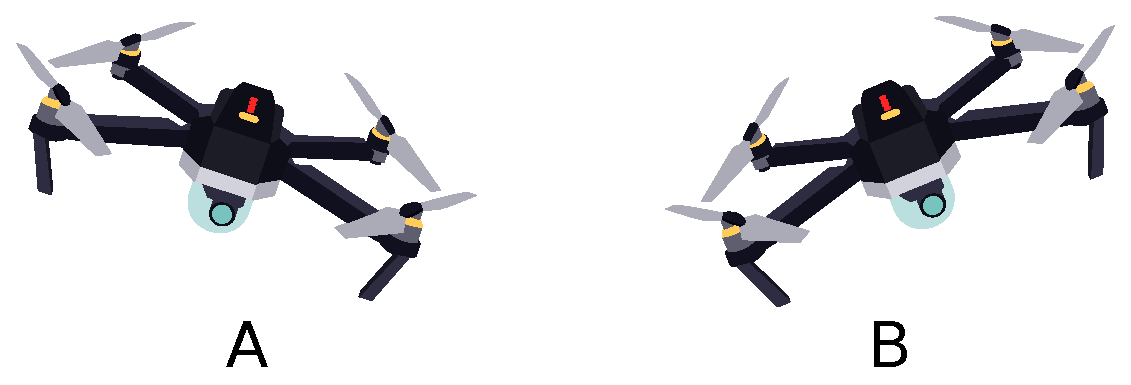
\includegraphics[width=0.55\textwidth]{Contenido/Cuerpo/Capitulo3/Fig10.eps}
	\captionof{figure}{Desplazamiento cuerpo rigido}
	\label{fig:ModeloMat:Fig1}
\end{center}
En el marco A, podemos encontrar 3 vectores linealmente independientes $a_1$, $a_2$ y $a_3$
y de la misma manera en el marco B tenemos tres vectores $b_1$, $b_2$ y $b_3$, podemos
escribir cualquier vector como una combinación lineal del vector base en cualquier marco
\begin{equation}
	\textbf{v} = v_1 \textbf{a}_1 + v_2 \textbf{a}_2 + v_3 \textbf{a}_3
\end{equation}
Tales vectores pueden ser vistos como ortogonales y si aplicamos una rotación del marco A
la transformación g queda ilustrada en la siguiente figura.
\begin{center}
	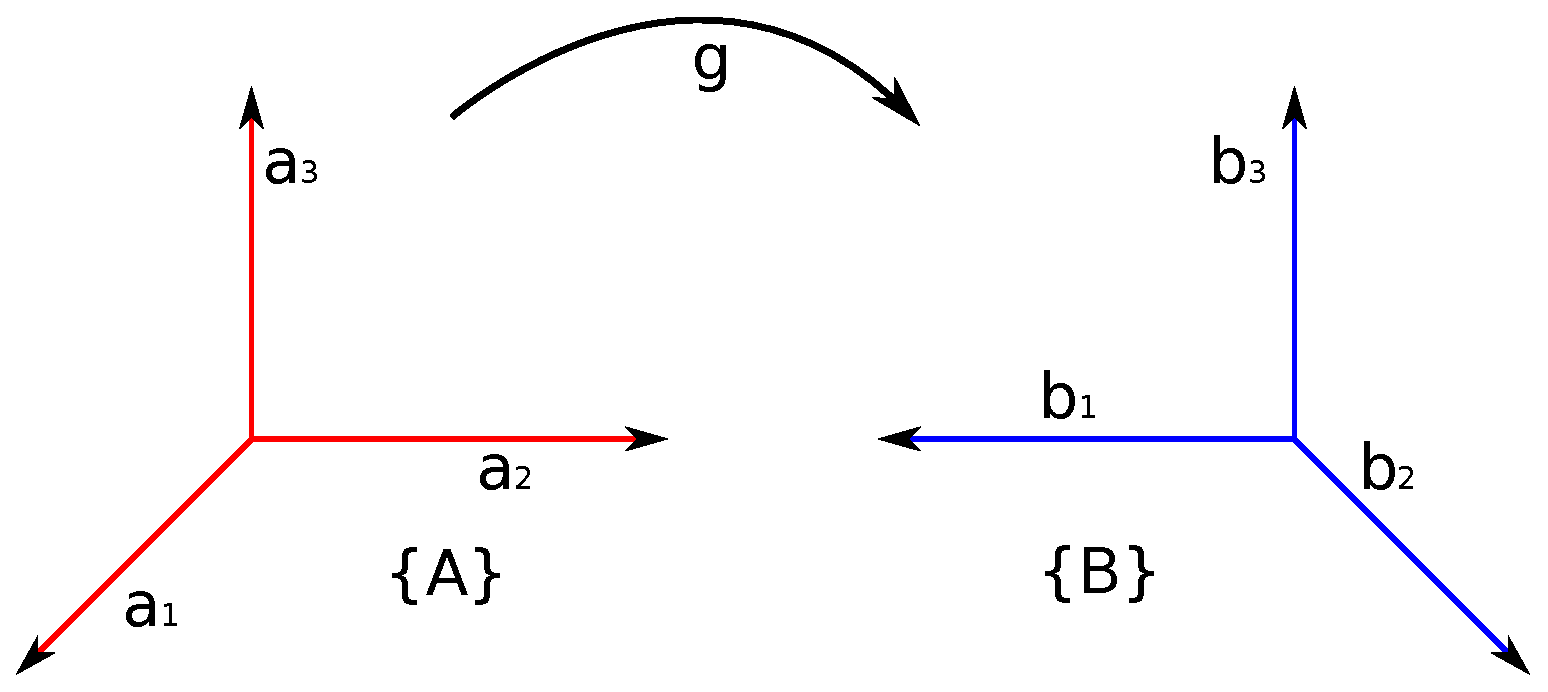
\includegraphics[width=0.55\textwidth]{Contenido/Cuerpo/Capitulo3/Fig11.eps}
	\captionof{figure}{Desplazamiento cuerpo rigido}
	\label{fig:ModeloMat:Fig1}
\end{center}
Podemos escribir ambos vectores ortogonales unitarios en un solo marco de referencia como
una combinacipon lineal de ambos
\begin{subequations}
	\begin{equation}
		\textbf{b}_1 = R_{11}\textbf{a}_1 + R_{12}\textbf{a}_2 + R_{13}\textbf{a}_3
	\end{equation}
	\begin{equation}
		\textbf{b}_2 = R_{21}\textbf{a}_1 + R_{22}\textbf{a}_2 + R_{23}\textbf{a}_3
	\end{equation}
	\begin{equation}
		\textbf{b}_3 = R_{31}\textbf{a}_1 + R_{32}\textbf{a}_2 + R_{33}\textbf{a}_3
	\end{equation}
\end{subequations}
Para este caso se escoge \textbf{b}$_1$, \textbf{b}$_2$ y \textbf{b}$_3$ como la combinación
lineal para \textbf{a}$_1$, \textbf{a}$_2$ y \textbf{a}$_3$ y los coeficientes de R se
pueden acomodar en un arreglo de 3x3 llamada matriz de rotación
\begin{equation}
	R=
	\begin{bmatrix}
		R_{11} & R_{12} & R_{13} \\
		R_{21} & R_{22} & R_{23} \\
		R_{31} & R_{32} & R_{33}
	\end{bmatrix}
\end{equation}
Y las propiedades de esta matriz son las siguientes
\begin{itemize}
	\item Ortogonal
	\item Su determínate es +1
	\item El producto de dos matrices de rotación da como resultado otra matriz de rotación
	\item La inversa de una matriz de rotación es también una matriz de rotación
\end{itemize}
La importancia de las matrices de rotación radican en que con ayuda de software y hardware
podemos aplicar técnicas de mapeo y simulación, además de que para el sistema de la gimbal
entra en juego múltiples marcos de referencia que constantemente cambian su orientación y
desplazamiento.\\
Ahora bien si trazamos un vector Q en cada marco de referencia como en la siguiente imagen
\begin{center}
	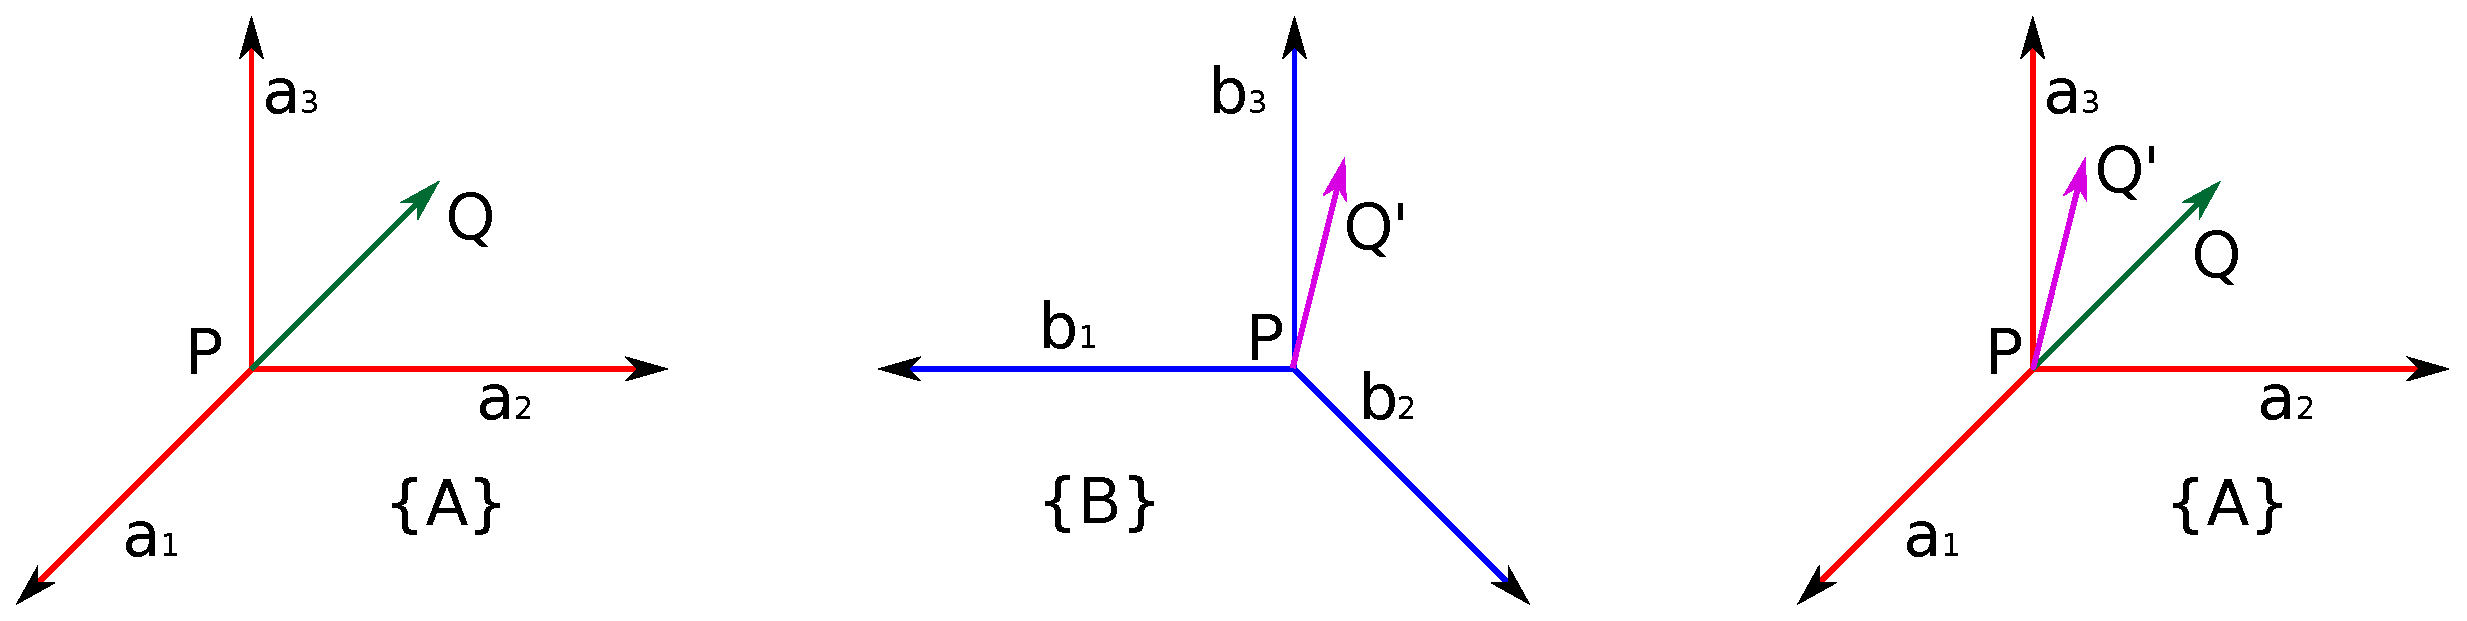
\includegraphics[width=0.75\textwidth]{Contenido/Cuerpo/Capitulo3/Fig12.eps}
	\captionof{figure}{Vectores de rotación}
	\label{fig:ModeloMat:Fig1}
\end{center}
Si trasladamos el marco B en A podremos obtener de nuevo una combinación lineal pero con
diferentes conjuntos de coeficientes
\begin{equation}
	\overrightarrow{PQ} = q_1\textbf{a}_1 + q_2\textbf{a}_2 + q_3\textbf{a}_3
\end{equation}
\begin{equation}
	\overrightarrow{PQ'} = q'_1\textbf{a}_1 + q'_2\textbf{a}_2 + q'_3\textbf{a}_3
\end{equation}
La matriz que conecta $q_1$, $q_2$ y $q_3$ con $q'_1$ , $q'_2$ y $q'_3$ es la matriz de
rotación vista en la ecuación 3.3
\begin{equation}
	\begin{bmatrix}
		q_1 \\
		q_2 \\
		q_3
	\end{bmatrix}
	=
	\begin{bmatrix}
		R_{11} & R_{12} & R_{13} \\
		R_{21} & R_{22} & R_{23} \\
		R_{31} & R_{32} & R_{33}
	\end{bmatrix}
	\begin{bmatrix}
		q'_1 \\
		q'_2 \\
		q'_3
	\end{bmatrix}
\end{equation}
Dicha matriz nos dice como se transforman los vectores de un marco de referencia a otro. La matrices
de rotación nos van a servir, como se mencionó anteriormente, para poder hacer mapeos del entorno, por
lo que necesitamos primero definir los marcos de referencia inercial y del cuerpo para posteriormente
hacer sus matrices de transformación.

% Los movimientos de la gimbal se basan en las coordenadas horizontales de azimuth y elevación, para gimbal de 3 grados de libertad
% se agrega un tercer eje cuyo movimiento se conoce como roll. El eje de azimuth y la elevación se visualizan más fácilmente al
% pensar en la posición de un objeto en relación con el horizonte.
% \begin{center}
% 	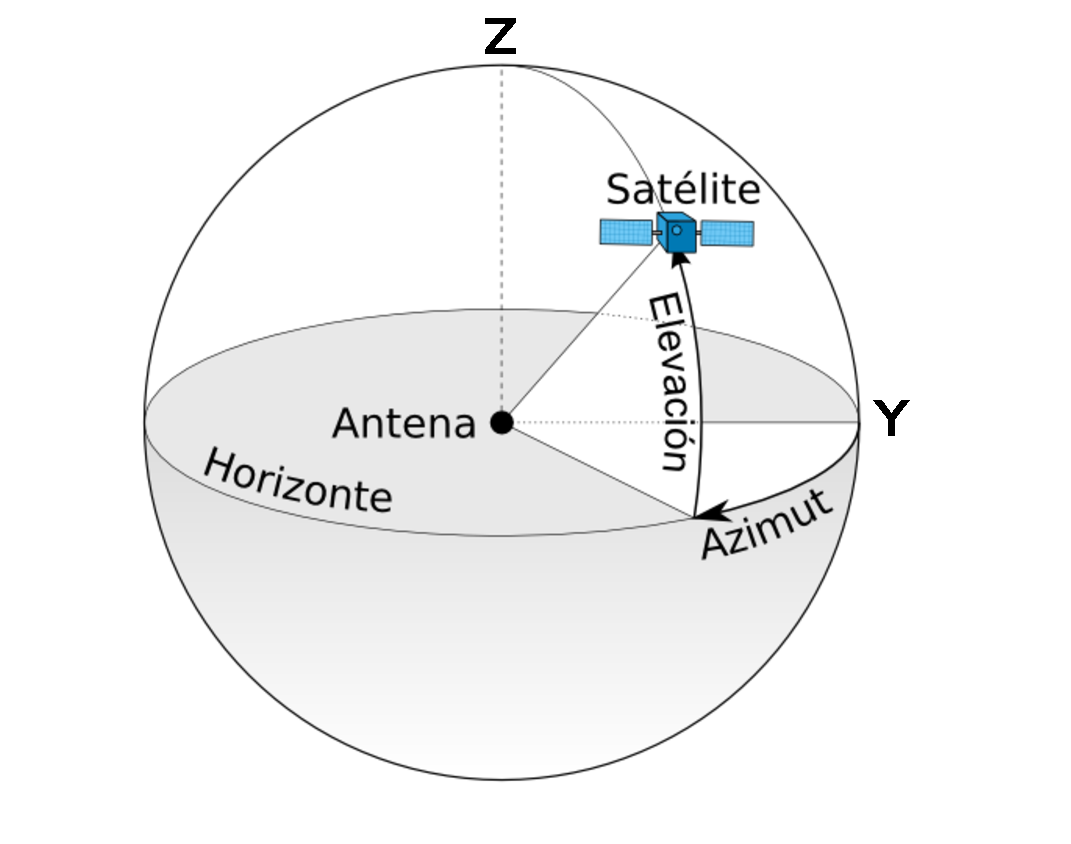
\includegraphics[width=0.55\textwidth]{Contenido/Cuerpo/Capitulo3/Fig1.eps}
% 	\captionof{figure}{Angulo de azimuth}
% 	\label{fig:ModeloMat:Fig1}
% \end{center}
% El angulo de azimuth es la posición alrededor del horizonte, medida desde un punto de referencia como el norte verdadero o el sur
% verdadero. Los movimientos de azimuth ocurren alrededor del eje Z (vertical).

% La elevación es la distancia del objeto por encima o por debajo del horizonte (también conocida como altitud en aplicaciones de
% astronomía y aeroespaciales). Los movimientos de elevación ocurren alrededor del eje Y.

% Los movimientos de balanceo ocurren alrededor del eje X a medida que gira con los ejes Y y Z.\\
% El control que se hace en la gimbal está dado por un motor con control de posición y una IMU (sensor inercial).Dicha gimbal esta
% montada en la parte delantera del vehículo aéreo como se muestra en la siguiente figura.
% \begin{center}
% 	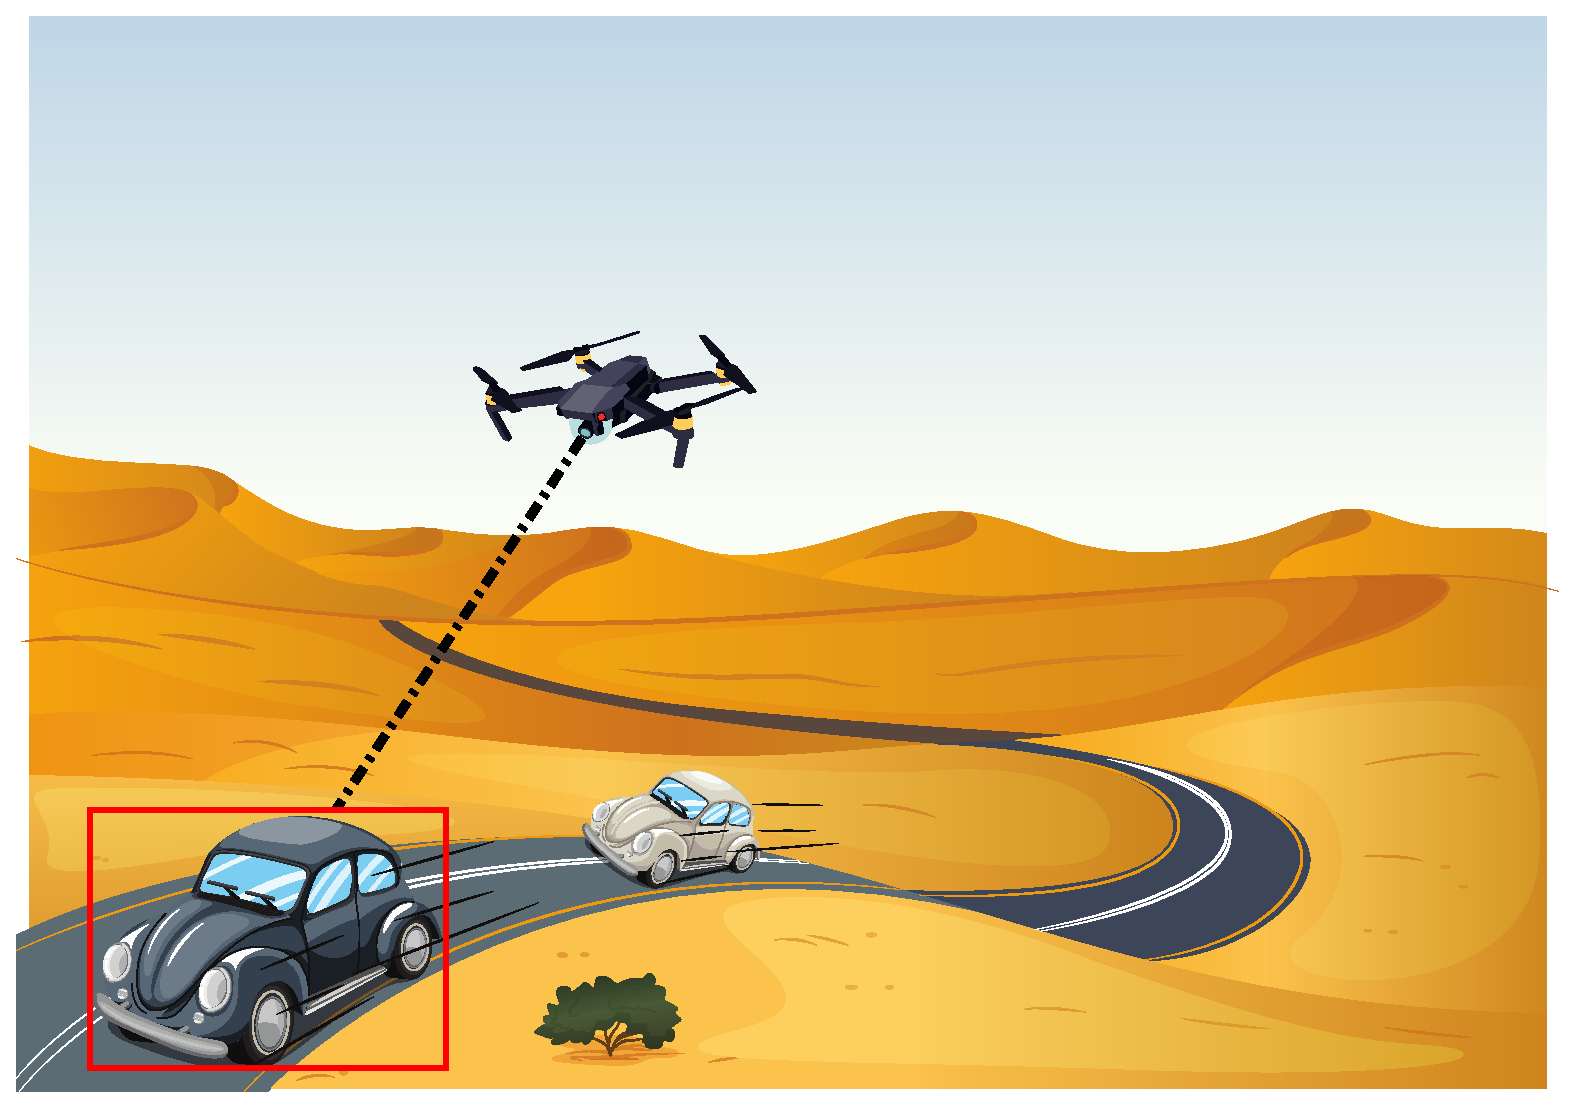
\includegraphics[width=0.55\textwidth]{Contenido/Cuerpo/Capitulo3/Fig2.eps}
% 	\captionof{figure}{Seguimiento de un objetivo utilizando una cámara sujeta a una gimbal embebida en un vehículo aéreo no tripulado.}
% 	\label{fig:ModeloMat:Fig1}
% \end{center}

\subsection{Marco de referencia Inercial [I]}
Antes de abordar el control de la gimbal, es necesario y obvio conocer el comportamiento
de dicho sistema, empezaremos por definir el marco de referencia inercial, es decir
el de la tierra. La siguiente imagen ilustra los ejes de este marco.
\begin{center}
	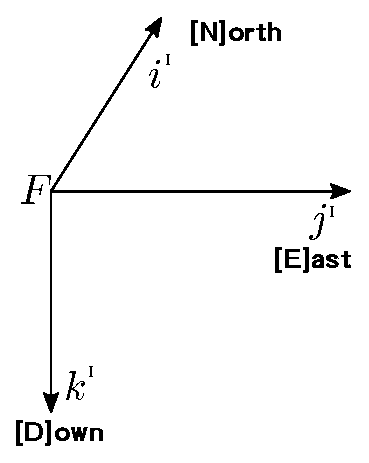
\includegraphics[width=0.25\textwidth]{Contenido/Cuerpo/Capitulo3/Fig4.eps}
	\captionof{figure}{Marco de referencia inercial}
	\label{fig:ModeloMat:Fig1}
\end{center}
Donde definimos a k apuntando hacia el centro de la tierra, este sistema de coordenadas
refieren a (Norte, Este y Abajo) de ahí su nombre NED(siglas en inglés).

\subsection{Marco de referencia del cuerpo [B]}
Una aeronave tiene la libertad de rotar en 3 ejes, en la aeronáutica son conocidos como
Yaw, Pitch y Roll. Dichas rotaciones son importantes en el control de aeronaves ya
que sirven para conocer la dinámica del sistema, dicha rotaciones pueden ser mejor
detalladas en una imagen, por lo que en la siguiente ilustración se grafica un plano
y se asigna nombre a cada rotación de los ejes.
\begin{center}
	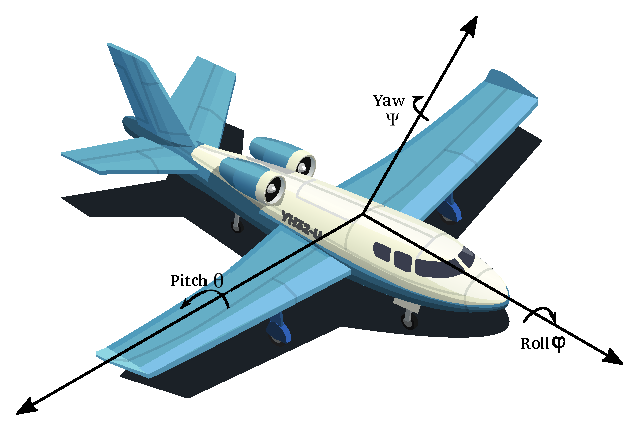
\includegraphics[width=0.35\textwidth]{Contenido/Cuerpo/Capitulo3/Fig6.eps}
	\captionof{figure}{Rotación en 3 ejes.}
	\label{fig:ModeloMat:Fig1}
\end{center}
Vamos a llamar marco de referencia del cuerpo a las coordenadas del UAV, es necesario establecer el centro del plano en el
centro de masas de la aeronave, como se ilustra en la siguiente figura.
\begin{center}
	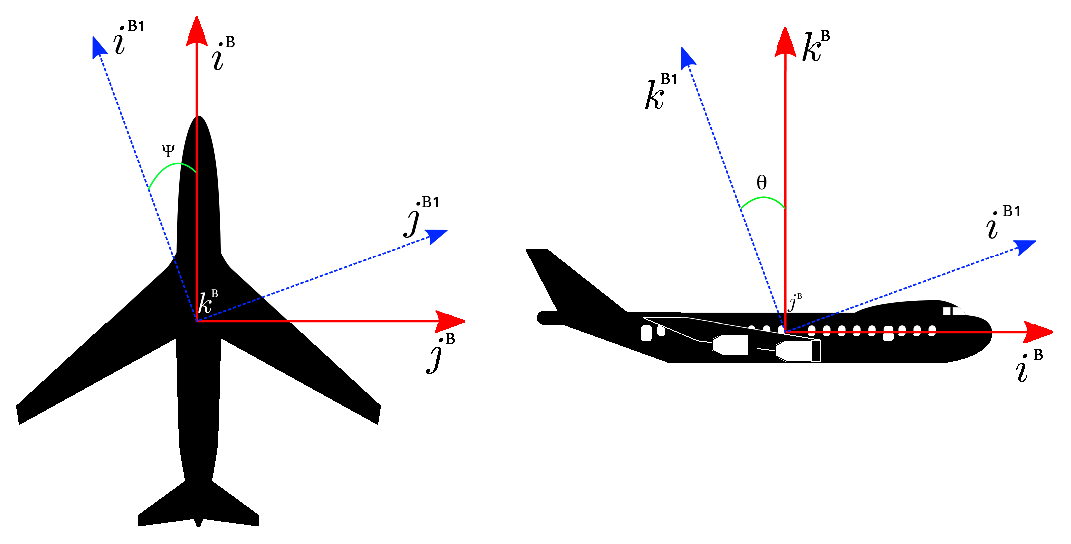
\includegraphics[width=0.5\textwidth]{Contenido/Cuerpo/Capitulo3/Fig5.eps}
	\captionof{figure}{Marco de referencia del cuerpo.}
	\label{fig:ModeloMat:Fig1}
\end{center}
De donde definimos las dos rotaciones que seran controladas en este trabajo pitch y yaw($\theta$, $\psi$). El subíndice B hace referencia
a Body y nos indica que estamos hablando de las coordenadas del UAV.

\subsection{Marco de referencia de la gimbal [G]}
Un último paso es definir un marco de referencia para la cámara, considerando que la cámara se encuentra en la parte delantera de
la aeronave y que el centro de la gimbal es el origen.
\begin{center}
	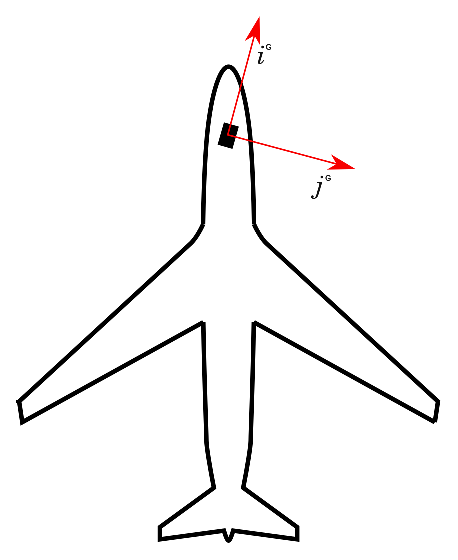
\includegraphics[width=0.3\textwidth]{Contenido/Cuerpo/Capitulo3/Fig7.eps}
	\captionof{figure}{Marco de referencia del la cámara.}
	\label{fig:ModeloMat:Fig1}
\end{center}
De donde el subíndice G hace referencia a que estamos en el plano de la gimbal. El vector unitario K apunta hacia afuera,
es decir hacia nosotros.

% ---------------------------------------------------------------------------------------------------------
% *********************************************************************************************************
% *********************************************************************************************************
% ---------------------------------------------------------------------------------------------------------

\section{Matrices de rotación}
Considerando el marco de referencia del cuerpo(B) y el de la Gimbal(G) tenemos los puntos Q y Q'
como se ilustra en la siguiente imagen
\begin{center}
	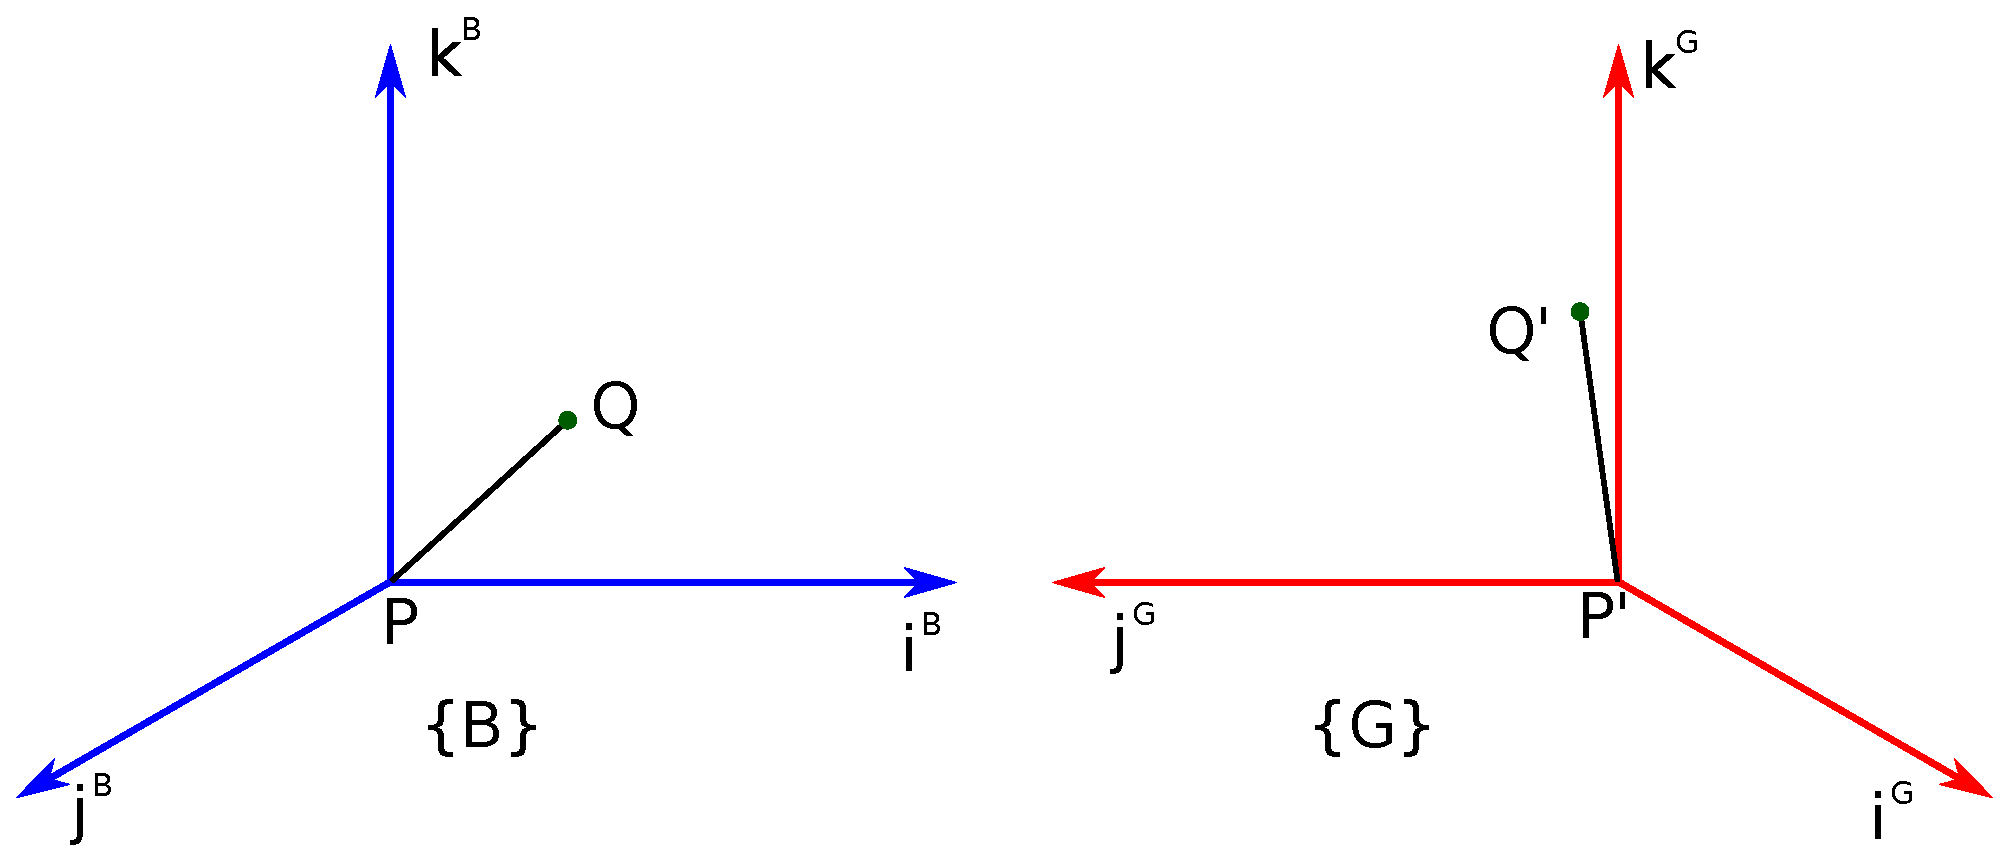
\includegraphics[width=0.75\textwidth]{Contenido/Cuerpo/Capitulo3/Fig13.eps}
	\captionof{figure}{Marco de referencia Body y gimbal}
	\label{fig:ModeloMat:Fig1}
\end{center}
Que podemos expresarlo en una combinación lineal para $\overrightarrow{PQ}$ y para $\overrightarrow{P'Q'}$
\begin{subequations}
	\begin{equation}
		PQ = q_1i^B + q_2j^B + q_3k^B
	\end{equation}
	\begin{equation}
		P'Q' = q_1i^G + q_2j^G + q_3k^G
	\end{equation}
\end{subequations}
Trasladamos el marco de referencia del gimbal en el del cuerpo
\begin{center}
	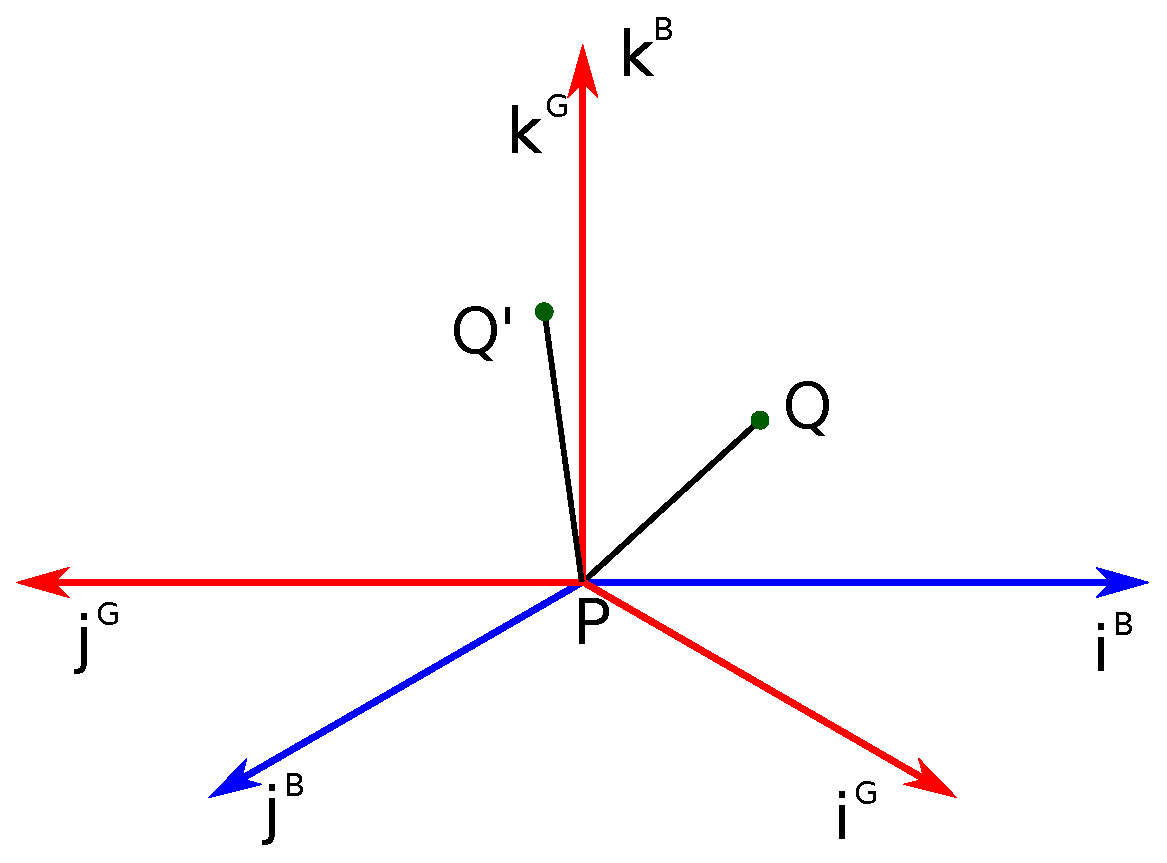
\includegraphics[width=0.45\textwidth]{Contenido/Cuerpo/Capitulo3/Fig14.eps}
	\captionof{figure}{Marco de referencia del gimbal trasladado en el del cuerpo}
	\label{fig:ModeloMat:Fig1}
\end{center}
Ahora tenemos un punto Q'' que es el punto Q' trasladado en el marco de referencia del cuerpo
\begin{equation}
	PQ'' = q_1i^B + q_2j^B + q_3k^B = q_1''i^G + q_2''j^G + q_3''k^G
\end{equation}
\begin{equation}
	\begin{bmatrix}
		q_1'' \\
		q_2'' \\
		q_3''
	\end{bmatrix}
	=
	\begin{bmatrix}
		R_{11} & R_{12} & R_{13} \\
		R_{21} & R_{22} & R_{23} \\
		R_{31} & R_{32} & R_{33}
	\end{bmatrix}
	\begin{bmatrix}
		q_1 \\
		q_2 \\
		q_3
	\end{bmatrix}
\end{equation}
La rotación sobre el eje k queda de la siguiente manera
\begin{center}
	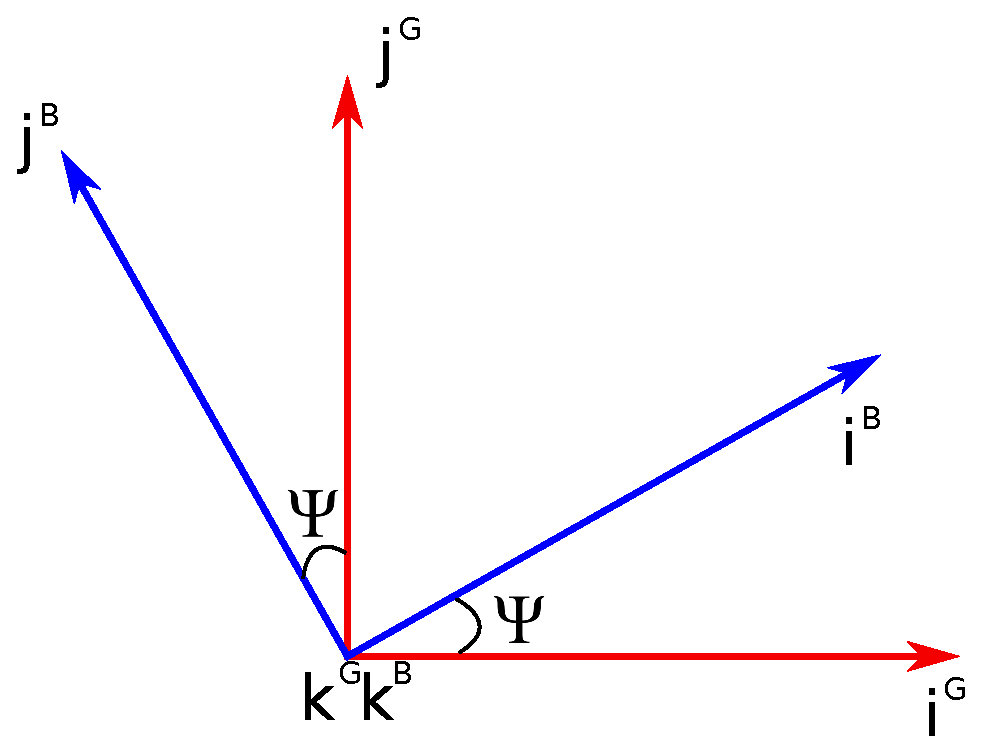
\includegraphics[width=0.45\textwidth]{Contenido/Cuerpo/Capitulo3/Fig15.eps}
	\captionof{figure}{Rotación en el eje k}
	\label{fig:ModeloMat:Fig1}
\end{center}
Se obtiene el cambio para $j^B$ y $i^B$
\begin{equation}
	i^B = |i^B|cos(\psi)i^G + |i^B|sin(\psi)j^G = cos(\psi)i^G + sin(\psi)j^G
\end{equation}
\begin{equation}
	j^B = -|j^B|sin(\psi)i^G + |j^B|cos\psi)j^G = -sin(\psi)i^G + cos(\psi)j^G
\end{equation}
Y de la ecuación 3.8 sustituimos $j^B$ y $i^B$
\begin{equation}
	PQ'' = q_1(cos(\psi)i^G + sin(\psi)j^G) + q_2(-sin(\psi)i^G + cos(\psi)j^G) + q_3(k^G)
\end{equation}
Simplificando la ecuación anterior tenemos
\begin{equation}
	PQ''= (q_1cos(\psi) - q_2sin(\psi))i^G + (q_1sin(\psi) + q_2cos(\psi))j^G + q_3(k^G)
\end{equation}
Y acomodando al ecuación 3.13 en matrices tenemos
\begin{equation}
	\begin{bmatrix}
		q_1'' \\
		q_2'' \\
		q_3''
	\end{bmatrix}
	=
	\begin{bmatrix}
		cos(\psi) & -sin(\psi) & 0 \\
		sin(\psi) & cos(\psi)  & 0 \\
		0         & 0          & 1
	\end{bmatrix}
	\begin{bmatrix}
		q_1 \\
		q_2 \\
		q_3
	\end{bmatrix}
\end{equation}
Ahora si rotamos sobre el eje x como se muestra en la siguiente figura
\begin{center}
	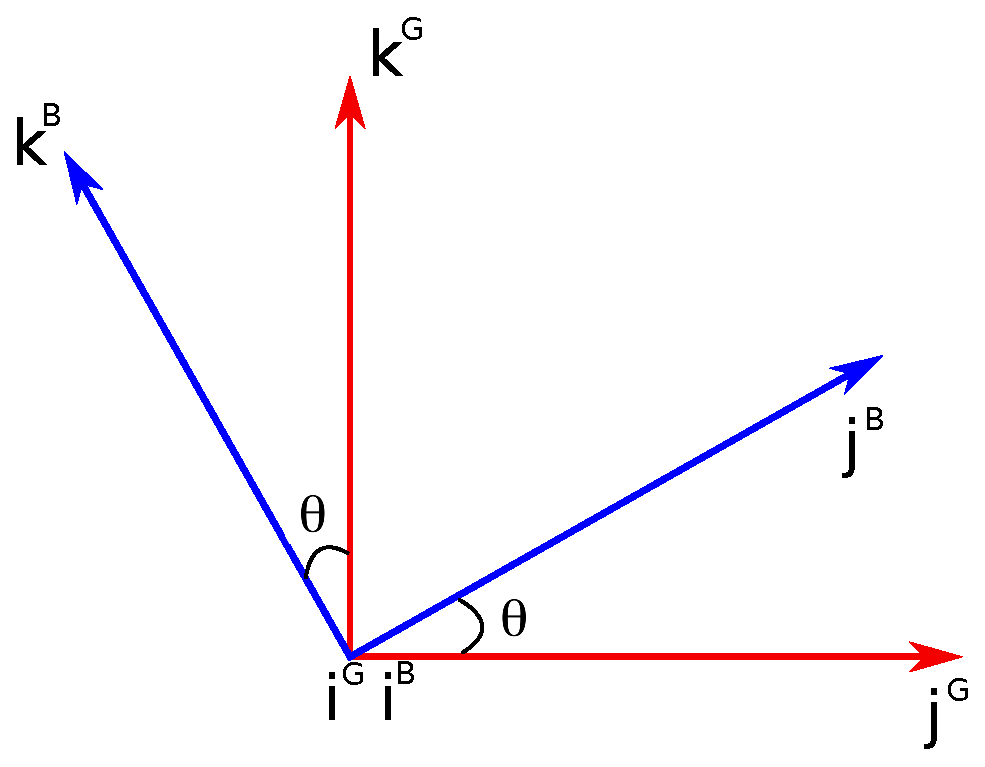
\includegraphics[width=0.45\textwidth]{Contenido/Cuerpo/Capitulo3/Fig17.eps}
	\captionof{figure}{Rotación en el eje x}
	\label{fig:ModeloMat:Fig1}
\end{center}
Se obtiene el cambio para $j^B$ y $k^B$
\begin{equation}
	j^B = |j^B|cos(\theta)j^G + |j^B|sin(\theta)k^G = cos(\theta)j^G + sin(\theta)k^G
\end{equation}
\begin{equation}
	k^B = -|k^B|sin(\theta)j^G + |k^B|cos\theta)k^G = -sin(\theta)j^G + cos(\theta)k^G
\end{equation}
Y de la ecuación 3.8 sustituimos $j^B$ y $k^B$
\begin{equation}
	PQ'' = q_1(i^G) + q_2(cos(\theta)j^G + sin(\theta)k^G) + q_3(-sin(\theta)j^G + cos(\theta)k^G)
\end{equation}
Simplificando la ecuación anterior tenemos
\begin{equation}
	PQ''= q_1(i^G) + (q_2cos(\theta) - q_3sin(\theta))j^G + (q_2sin(\theta) + q_3cos(\theta))k^G
\end{equation}
Y acomodando al ecuación 3.18 en matrices tenemos
\begin{equation}
	\begin{bmatrix}
		q_1'' \\
		q_2'' \\
		q_3''
	\end{bmatrix}
	=
	\begin{bmatrix}
		1 & 0           & 0            \\
		0 & cos(\theta) & -sin(\theta) \\
		0 & sin(\theta) & cos(\theta)
	\end{bmatrix}
	\begin{bmatrix}
		q_1 \\
		q_2 \\
		q_3
	\end{bmatrix}
\end{equation}



% Poniendo en el mismo plano dos referencias, el de la gimbal y el del body, tal como se ilustra en la siguiente figura
% \begin{center}
% 	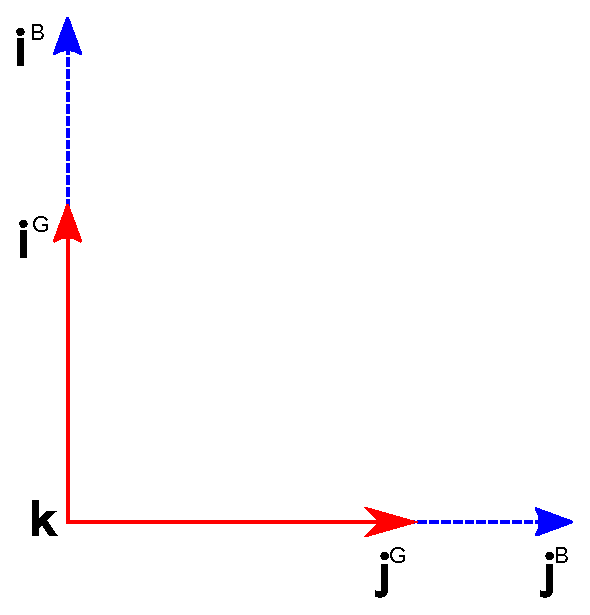
\includegraphics[width=0.3\textwidth]{Contenido/Cuerpo/Capitulo3/Fig8.eps}
% 	\captionof{figure}{Marco de referencia Body y gimbal}
% 	\label{fig:ModeloMat:Fig1}
% \end{center}
% Cualquier punto en el plano puede ser expresado como:
% \begin{equation}
% 	p_{i^B,j^B} = [p_i^B , p_j^B]^T = p_i i^B + p_j p^B
% \end{equation}
% \begin{equation}
% 	p_{i^G,j^G} = [p_i^G , p_j^G]^T = p_i \cdot i^G + p_j\cdot  p^G
% \end{equation}
% \begin{equation}
% 	\textbf{P}_{i,j}^B = \textbf{P}_{i,j}^G
% \end{equation}

% Si hacemos rotar el frame de la gimbal respecto al eje K obtenemos que:
% \begin{center}
% 	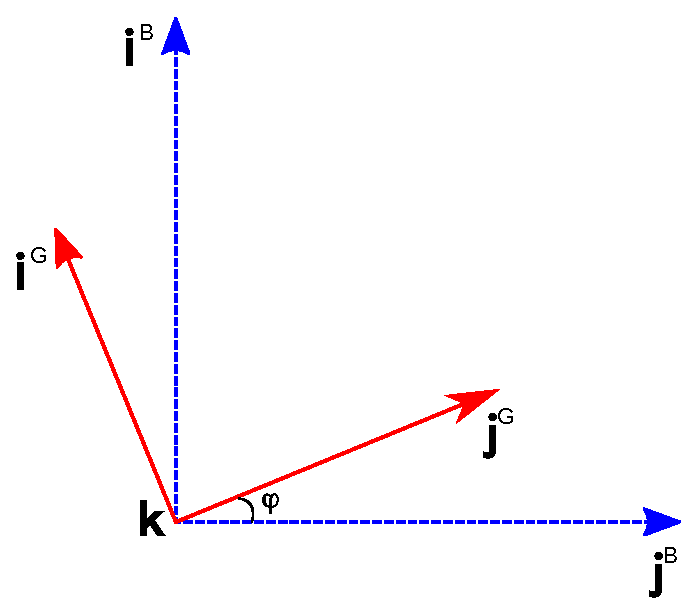
\includegraphics[width=0.3\textwidth]{Contenido/Cuerpo/Capitulo3/Fig9.eps}
% 	\captionof{figure}{Rotación del marco de referencia Gimbal respecto al del cuerpo}
% 	\label{fig:ModeloMat:Fig1}
% \end{center}
% \begin{equation}
% 	p_{i^B,j^B} = [p_i^B , p_j^B]^T = p_i i^B + p_j p^B
% \end{equation}
% \begin{equation}
% 	p_{i^G,j^G} = [p_i^G , p_j^G]^T = p_i i^G + p_j p^G
% \end{equation}
% Como
% \begin{equation}
% 	p_i = p_{i,j}^G \cdot i^B = p_i^G i^B \cdot i^G + p_j^G i^B \cdot j^G
% \end{equation}
% \begin{equation}
% 	p_j = p_{i,j}^G \cdot j^B = p_i^G j^B \cdot i^G + p_j^G j^B \cdot j^G
% \end{equation}
% Entonces
% \begin{equation*}
% 	\begin{bmatrix}
% 		p_i^B \\
% 		p_j^B
% 	\end{bmatrix}
% 	=
% 	R
% 	\begin{bmatrix}
% 		p_i^G \\
% 		p_j^G
% 	\end{bmatrix}
% \end{equation*}
% Donde la matriz de rotación etsa dada por:
% \begin{equation*}
% 	R=
% 	\begin{bmatrix}
% 		i^B\cdot i^G & i^B \cdot j^G \\
% 		j^B\cdot i^G & j^B \cdot j^G
% 	\end{bmatrix}
% 	=
% 	\begin{bmatrix}
% 		cos(\psi) & -sin(\psi) \\
% 		sin(\psi) & cos(\psi)
% 	\end{bmatrix}
% \end{equation*}

% ---------------------------------------------------------------------------------------------------------
% *********************************************************************************************************
% *********************************************************************************************************
% ---------------------------------------------------------------------------------------------------------
\section{Modelo matemático del motor DC}
El mecanismo móvil del sistema esta conformado por un par de motores de corriente directa, como vimos
en el capítulo 2 para poder hacer diseñar un controlador necesitamos primero obtener la ecuación dinámica
del sistema, en este caso la ecuación dinámica del motor.\\
La siguiente figura muestra el diagrama electrico de un motor de corriente directa
\begin{center}
	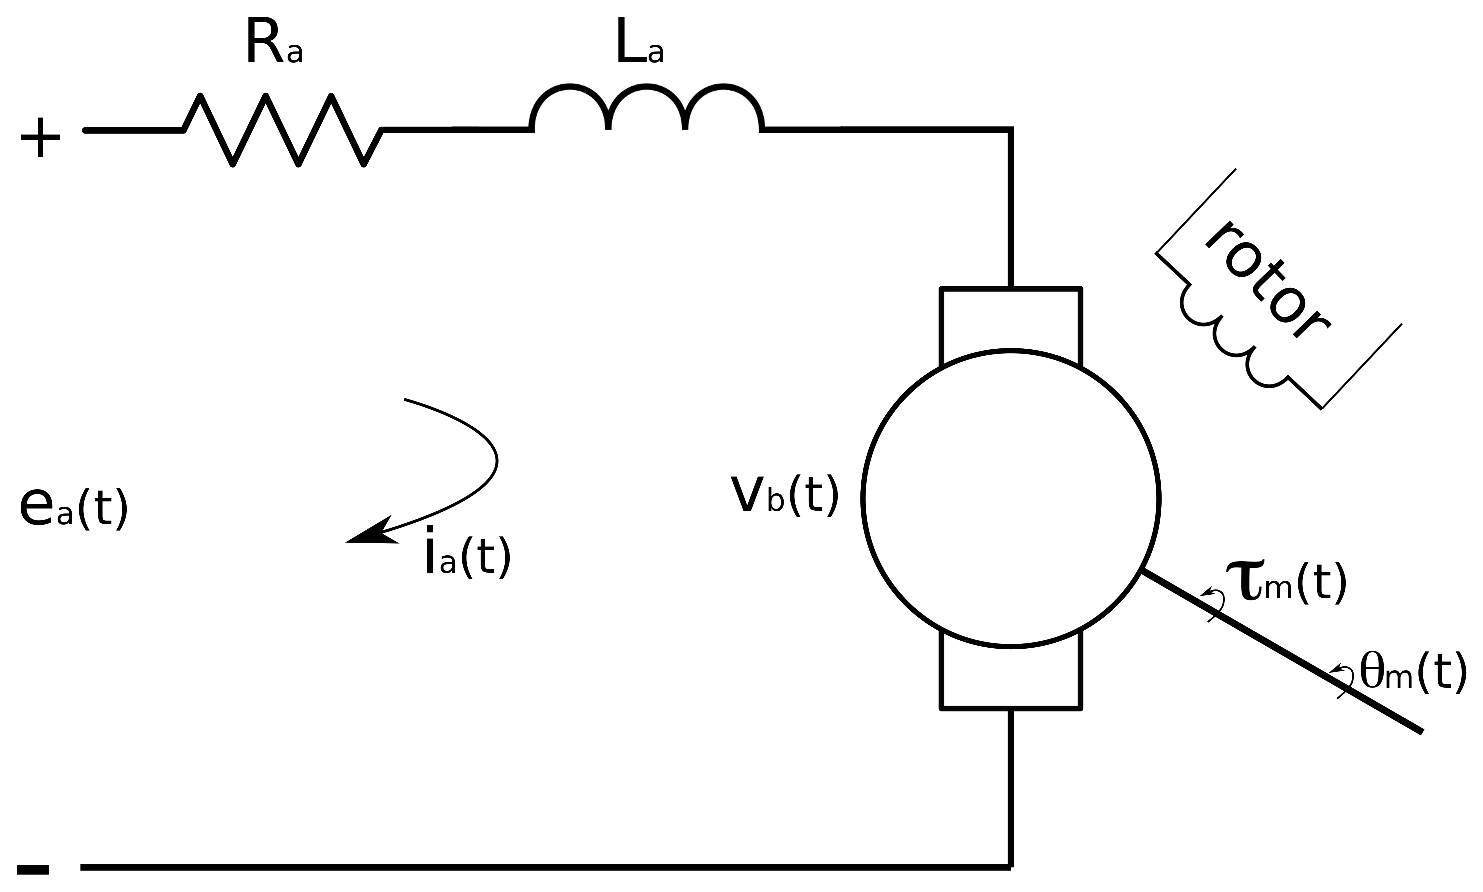
\includegraphics[width=0.5\textwidth]{Contenido/Cuerpo/Capitulo3/Fig16.eps}
	\captionof{figure}{Diagrama electrico de motor de corriente directa}
	\label{fig:ModeloMat:Fig1}
\end{center}
Tenemos que la fuerza contra motriz $v_b$ es igual a la siguiente ecuación
\begin{equation}
	v_b(t) =K_b \frac{d\theta_m(t)}{dt}
\end{equation}
donde
\begin{itemize}
	\item $ \frac{d\theta_m(t)}{dt} $ = $ \omega_m(t) $
\end{itemize}
Aplicamos laplace a la ecuación anterior
\begin{equation}
	V_b(s) = K_bS\Theta_m(s)
\end{equation}
Aplicando la ley de Kirkoff a la red eléctrica de la figura 3.11 obtenemos
\begin{equation}
	R_aI_a(s) + L_aSI_a(s) + V_b(s) = E_a(s)
\end{equation}
El torque empleado por el motor es proporcional a la corriente del inducido; por lo tanto,
\begin{equation}
	\tau_m(s) = K_\tau I_a(s)
\end{equation}
donde $\tau_m$ es el torque del motor y $K_\tau$ es una constante de proporcionalidad, llamada constante de par del motor, que depende de las características del motor y del
campo magnético.\\
En un arreglo consistente de unidades, el valor de $K_t$ es igual al valor de $K_b$. Reordenando la ecuación 3.18.
\begin{equation}
	I_a = \frac{1}{K_\tau} \tau_m (s)
\end{equation}
Para encontrar la función de transferencia del motor, primero sustituimos las ecuaciones (3.16) y (3.19) en (3.17), produciendo
\begin{equation}
	\frac{(R_a + L_aS) \tau_m(s)}{K_\tau} + K_bS \Theta_m(s) = E_a(s)
\end{equation}
El torque del motor puede ser expresado como
\begin{equation}
	\tau_m(s) = (J_mS^2 + D_mS) \Theta_m(s)
\end{equation}
$J_m$ es la inercia equivalente en la armadura e incluye tanto la inercia de la armadura como la inercia de carga reflejada en la armadura. $D_m$ es la amortiguación viscosa
equivalente en la armadura e incluye tanto la amortiguación viscosa de la armadura como la amortiguación viscosa de la carga reflejada en la armadura.\\
Sustituyendo $\tau_m$ en la ecuación 3.2 obtenemos
\begin{equation}
	\frac{(R_a + L_aS) (J_mS^2 + D_mS) \Theta_m(s) }{K_\tau} + K_bS \Theta_m(s) = E_a(s)
\end{equation}
Si suponemos que la inductancia de la armadura, $L_a$, es pequeña en comparación con la resistencia de la armadura, $R_a$, que es habitual para un motor de corriente continua,
la ecuación. (3.22) se convierte
\begin{equation}
	\left[ \frac{R_a }{K_\tau} (J_mS^2 + D_mS) + k_b \right] S\Theta_m(s)  = E_a(s)
\end{equation}
Después de la simplificación, se encuentra que la función de transferencia deseada,
\begin{equation}
	\frac{\theta_m (s)}{E_a(s)} = \frac{K_t / (R_aJ_m)}{s \left[ s + \frac{1}{J_m} \left( D_m + \frac{K_tK_b}{R_a} \right) \right]}
\end{equation}
Que en manera simple se obtiene.
\begin{equation}
	\frac{\theta_m (s)}{E_a(s)} = \frac{K}{s(s+\alpha)}
\end{equation}
Discutamos primero las constantes mecánicas, $J_m$ y $D_m$. Considere la siguiente figura, que muestra un motor con inercia $J_a$
y amortiguación $D_a$ en la armadura que impulsa una carga que consiste en inercia $J_L$ y amortiguación $D_L$
\begin{center}
	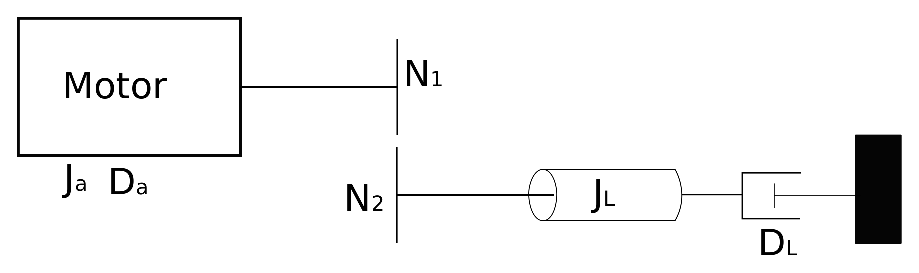
\includegraphics[width=0.5\textwidth]{Contenido/Cuerpo/Capitulo3/Fig18.eps}
	\captionof{figure}{Motor DC que acciona una carga mecánica rotacional}
	\label{fig:ModeloMat:Fig1}
\end{center}
Suponiendo que se conocen todos los valores de inercia y amortiguación mostrados, $J_L$ y $D_L$ pueden reflejarse de nuevo en la
armadura como una inercia y amortiguación equivalentes para agregarse a $J_a$ y $D_a$, respectivamente. Por lo tanto, la inercia
equivalente, $J_m$, y la amortiguación equivalente, $D_m$, en la armadura son
\begin{subequations}
	\begin{equation}
		J_m = J_a + J_L \left( \frac{N_1}{N_2} \right)
	\end{equation}
	\begin{equation}
		D_m = D_a + D_L\left( \frac{N_1}{N_2} \right)
	\end{equation}
\end{subequations}
Ahora que hemos evaluado las constantes mecánicas, $J_m$ y $D_m$, tenemos que obtener las constantes electricas vistas en la
ecuación 3.29. Sustituyendo las ecuaciones (3.21) y (3.24) en la ecuación. (3.22), con $L_a = 0$, produce
\begin{equation}
	\frac{R_a}{K_t} \tau_m (s) + K_bS\theta_m(s) = E_a(s)
\end{equation}
Aplicando la transformada inversa de laplace obtenemos
\begin{equation}
	\frac{R_a}{K_t} \tau_m (t) + K_b\omega_m(t) = e_a(s)
\end{equation}
Si se aplica un voltaje de CC, $e_a$, el motor girará a una velocidad angular constante, $\omega_m$, con un torque constante,$\tau_m$.
Por lo tanto,podemos descartar la relación funcional basada en el tiempo de la ecuación (3.33), la siguiente relación existe
cuando el motor está funcionando en estado estable con una entrada de voltaje de CC:
\begin{equation}
	\frac{R_a}{K_t} \tau_m + K_b\omega_m = e_a
\end{equation}
La siguiente ecuación representa una linea recta de $\tau_m$ vs $\omega_m$
\begin{equation}
	\tau_m = -\frac{K_bK_t}{R_a} \omega_m + \frac{K_t}{R_a}e_a
\end{equation}
Este gráfico se llama curva de par-velocidad. La intersección del eje de torque ocurre cuando la velocidad angular llega a cero.
Ese valor de par se llama Torque "stall", $\tau_{stall}$.
\begin{center}
	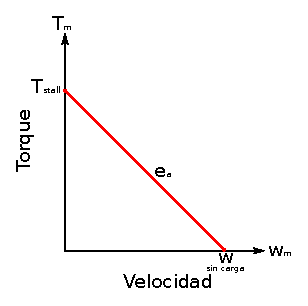
\includegraphics[width=0.45\textwidth]{Contenido/Cuerpo/Capitulo3/Fig19.eps}
	\captionof{figure}{Curva de par-velocidad}
	\label{fig:ModeloMat:Fig1}
\end{center}
Por tanto tenemos que
\begin{equation}
	T_{stall} = \frac{K_t}{R_a}e_a
\end{equation}
La velocidad angular que ocurre cuando el torque es cero se llama velocidad sin carga, $\omega_{sin carga}$ . Así,
\begin{equation}
	\omega_{sin carga} = \frac{e_a}{K_b}
\end{equation}
Las constantes eléctricas de la función de transferencia del motor ahora se pueden encontrar en las ecuaciones (3.36) y (3.37) como
\begin{equation}
	\frac{K_t}{R_a} = \frac{T_{stall}}{e_a}
\end{equation}
y 
\begin{equation}
	K_b = \frac{e_a}{\omega_{sincarga}}
\end{equation}